\section{Calculation von Neumann}
\begin{itemize}
\item
Firstly we calculate the vonNeumann entropy of a so-called maximally entangled state. As an experimental example we use the 2-qubit state:
\begin{equation}
|\psi\rangle=\frac{|H\rangle|x+\rangle-i|V\rangle|x-\rangle}{\sqrt{2}}
\label{psivon}
\end{equation}
from \cite{PhysRevLett.110.167401}. Here $\ket{H}$ and $\ket{V}$ denote the
horizontal and vertical polarization of light(first qubit) while $\ket{x\pm}$ are ground and excited states a singly charged superconductor quantum dot(second qubit). The convention is usually to denote as $\ket{0}$ the horizontal polarization and the down(minus) spin of the quantum dot. Hence the state is rewritten in the tensor product:
\begin{equation}
|\psi\rangle=\frac{|01\rangle-i|10\rangle}{\sqrt{2}}=\frac{1}{\sqrt{2}}\left(
\begin{array}{c}
 0 \\
 1\\
 -i\\
 0 \\
\end{array}
\right)
\label{pspspsps}
\end{equation}
Thus the density matrix is:
\begin{align}
\label{rhomatrix}
\rho &= \ket{\psi} \bra{\psi} \nonumber \\[0.5em]
&=\frac{1}{2}\big{(}|01\rangle-i|10\rangle\big{)}\big{(}\langle01|+i\langle10|\big{)}\\[0.5em]
&=\frac{1}{2}\left(
\begin{array}{cccc}
 0 & 0 & 0 & 0 \\
 0 & 1 & i & 0 \\
 0 & -i & 1 & 0 \\
 0 & 0 & 0 & 0 \\
\end{array}
\right)\nonumber
\end{align}
Now, we write the matrix $\rho$ using its modal matrix and the corresponding diagonal matrix. 
First we find the eigenvectors and eigenvalues  of $\rho$:
\begin{equation}
\lambda_1=1,\:  \lambda_2=0,\:  \lambda_3=0,\:  \lambda_4=0, 
\end{equation}
\begin{equation}
v_1=\left(
\begin{array}{c}
 0 \\
 i\\
 1\\
 0 \\
\end{array}
\right),
\:  v_2=\left(
\begin{array}{c}
 0 \\
 0\\
 0\\
 1 \\
\end{array}
\right),
\:  v_3= \left(
\begin{array}{c}
 0 \\
 -i\\
 1\\
 0 \\
\end{array}
\right),\:  v_4= 
\left(
\begin{array}{c}
 1 \\
 0\\
 0\\
 0 \\
\end{array}
\right)
\end{equation}
Now we readily see that the modal matrix is:
\begin{equation}
M=
\left( \begin{array}{cccc}
 0 & 0 & 0 & 1 \\
 i & 0 & -i & 0 \\
 1 & 0 & 1 & 0 \\
 0 & 1 & 0 & 0 \\
\end{array}
\right)
\end{equation}
which gives us $det(M)=2i$ and : 
\begin{equation}
M^{-1}=\frac{1}{2}
\left( \begin{array}{cccc}
 0 & -i & 1 & 0 \\
 0 & 0 & 0 & 2 \\
 0 & i & 1 & 0 \\
 2 & 0 & 0 & 0 \\
\end{array}
\right).
\end{equation}
From the modal matrices we diagonalize $\rho$:
\begin{equation}
\rho=MDM^{-1}
\end{equation}
in which:
\begin{equation}
D= \diag (1,0,0,0).
\label{diag}
\end{equation}
Now, using \propref{spectraltheorem} we apply \defref{vonNeumanndef} as prescribed, in order to calculate the von Neumann entropy:
\begin{align}
S(\rho) &= -\Tr (F(\rho))\label{functionimp:1} \\[0.5em] 
&= -\Tr (F(MDM^{-1})) \nonumber \\[0.5em]
&=-\Tr \Bigg[
M
\left( \begin{array}{cccc}
 F(1) & 0 & 0 & 0 \\
 0 & F(0) & 0 & 0 \\
 0 & 0 & F(0) & 0 \\
 0 & 0 & 0 & F(0) \\
\end{array}
\right)
M^{-1}
\Bigg]
\nonumber\\[0.5em]
&=0
\label{functionimp}
\end{align}  
The result is of course expected since the vonNeumman entropy is zero if and only if $\rho$ is a pure state.

\item
Let's calculate now the von Neumann entropy of a standard example (taken from page 504 of \citep{nielsen_chuang_2010}):
\begin{align}
\rho(s) & = s \ket{0} \bra{0} + (1-s) \ket{1} \bra{1} \\[0.5em] & =  \left(
\begin{array}{cc}
 s & 0 \\
 0 & 1-s \\
\end{array}
\right)
\label{ffrefer}
\end{align}
with $0<s<1$.
Since the density matrix is already diagonal, calculating the eigenvalues and eigenvectors becomes redundant. We directly apply \defref{vonNeumann2} and get:
\begin{align}
S(\rho(s)) &= - \Tr \left[ F(\rho(s))) \right] \\[0.5em] &=
-\Tr \bigg[ \left(
\begin{array}{cc}
 s \log (s) & 0 \\
 0 & (1-s) \log (1-s) \\[0.5em]
\end{array}
\right) \bigg] \\[0.5em]
&= -(1-s) \log (1-s)-s \log (s)
\end{align}

\begin{figure}
\begin{center}
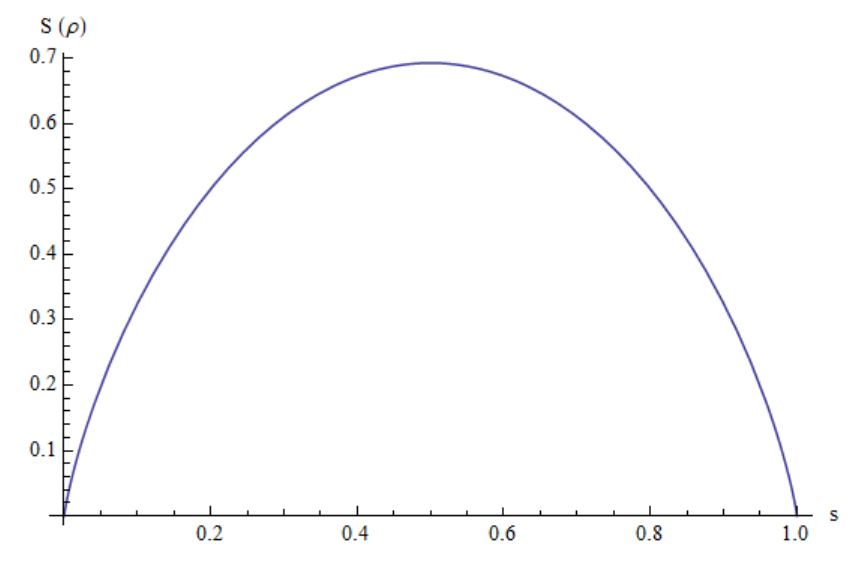
\includegraphics[scale=0.8]{figures/von_ent_plot.png}
\caption{Plotting it using the natural logarithm, demonstrates that the von Neumann entropy can measure the amount of departure from a pure state. For $s=0.5$ our state has the maximum departure from a pure state.}
\label{figure1}
\end{center}
\end{figure}

The physicality of this calculation becomes vivid, if we generalize this system to a statistical mixture of $N$ orthogonal(mutually exclusive) pure states. In the standard basis this will write:

\begin{align}
\label{asdasdas}
\rho &= \sum_{i=0}^{N-1}\rho_{i}\ket{i}\bra{i} \\[0.5em]
&= \diag (\rho_{0},\rho_{1},..,\rho_{N-2},\rho_{N-1})
\end{align}
which is an $N\times N$ diagonal matrix with \begin{equation}
\sum_{i=0}^{N-1}\rho_{i}=1
\end{equation}
Applying \defref{vonNeumanndef} we get:
\begin{align}
S(\rho) &= -\Tr \left[ \diag \big( F(\rho_{0}),F(\rho_{1}),..,F(\rho_{N-2}),F(\rho_{N-1})
 \big) \right] \\[0.5 em] &= -\sum_{i=0}^{N-1}\rho_{i} \log \rho_{i} \label{rrrrrrrrr}
\end{align}
It is easy to see the similarity with Shannon's information entropy \eqref{shanon}.
\par
Even though both information(quantum or not) and thermal entropy are generated via different methods(mathematically and conceptually), in a simple statistical mechanics problem these pure states can represent possible macrostates of a thermal system. 
\\*
For example a fixed temperature gas at a $T=1 / k_{B} \beta$ in a canonical ensemble model has a density operator:
\begin{equation}
\rho_{CE}=\frac{\exp (-\beta \hat{H})}{Z}
\end{equation}
with $\beta$ being a free parameter, $\hat{H}$ and  $\epsilon_{n}$ denotes the hamiltonian and its eigenvalues and $Z$ the quantum partition function:
\begin{equation}
Z=\Tr\left(\mathrm{e}^{-\beta \hat{H}}\right)=\sum_{i} \mathrm{e}^{-\beta \epsilon_{i}}
\end{equation}
based on the condition $\Tr(\rho)=1$. Thus each probability in \eqref{rrrrrrrrr} is:
\begin{equation}
\rho_{i}= e^{-\beta \epsilon_{i}}/Z
\end{equation}
\end{itemize}